\documentclass[11pt,oneside, a4paper]{report}
\usepackage{algorithm}
\usepackage[utf8]{inputenc}
\usepackage{mathtools}
\usepackage{graphicx}
\pagestyle{headings}

\begin{document}
\chapter{Modeling techniques}

\section{Decision trees}
A decision tree is a tree-like capable of classifying its inputs based on values of a set of chosen discrete-valued attributes (real-valued attributes must be first discretized). Each of the non-leaf nodes represents a test which determines the next node to visit while traversing the tree in a top-down fashion. The classification process is finished after reaching a leaf with a class label assigned to it.

An example of a decision tree is shown in Figure \ref{fig:decision-tree}. Its leaves symbolize the probability that a given person will buy a car within  5 years period.

\begin{figure}[htp]
\centering
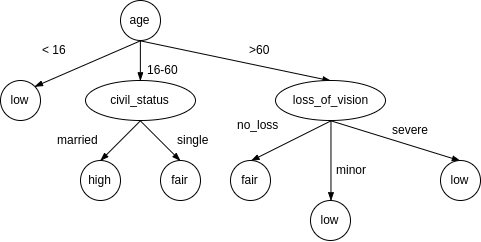
\includegraphics[scale=0.70]{figures/decision-tree.png}
\caption{An example of a decision tree}
\label{fig:decision-tree}
\end{figure}

\subsection{Tree induction}
Many algorithms for decision tree induction have been proposed. Some of the notable examples are: ID3 \cite{QUINLAN1986}, C4.5 \cite{QUINLAN1993} and RandomForest \cite{HO1995}. The basic idea behind them will be explained on the basis of descriptions of the ID3 algorithm that can be found in \cite{HAN2005} and \cite{QUINLAN1986}.
At the beginning it is necessary to identify an attribute C that will act as a criterion for specifying classes ${C_1, C_2, ... , C_m}$ that samples should be assigned to ($m$ is the number of distinct values that $C$ can take).
Next an attribute needs to be chosen in order to partition the data. The choice is made on the basis of the information gain. One of the factors that influence its value is the amount of information required to perform classification given by the expression

\begin{equation} \label{eq:information-gain}
I(s_1, s_2, ..., s_m) = - \sum_{i=1}^{m} p_i \log_{2}(p_i)
\end{equation}

where $s_i$ is the number of samples in the class $C_i$ and $p_i$ is the probability of a sample being a member of the $C_i$ class. The value of $p_i$ can be expressed as the ratio $\frac{s_i}{s}$ where $s$ is the number of all samples.
Let us assume that the currently considered attribute $A$ takes one of the $v$ following values: ${a_1, a_2, ..., a_v}$. The entropy, representing the expected information based on splitting the data by a tree with the attribute A as the root is formulated in the following way

\begin{equation} \label{eq:entropy}
E(A) = \sum_{j=1}^{v} \frac{s_{1j} + s_{2j} + ... + s_{mj}}{s} I(s_{1j}, ..., s_{mj})
\end{equation}

where $s_{ij}$ means the number of samples from the class $C_i$ having the attribute $A$ equal to $a_j$.
Finally the value of information gain for the attribute $A$ is given in the form

\begin{equation} \label{eq:information-gain}
Gain(A) = I(s_1, s_2, ... , s_m) - E(A)
\end{equation}

After computing the information gain for each attribute, the one with the highest value is chosen and a partition node is added to the tree. For each value ${a_1, a_2, ..., a_v}$ a new branch is created. Samples are split into groups based on their value of the chosen attribute. Then the whole process is repeated for each group of samples. If there are no samples with the value $a_i$, a leaf labeled with the class most frequent among samples is attached to that branch. Induction is continued until all the samples have been processed or there are no attributes left.

\section{Bayesian networks}
\section{Neural networks}
An artificial neural network (ANN) is a network comprised of connected processing units called neurons. A neuron is capable of calculating a linear combination of its inputs and an additional parameter called bias. The output of a neuron is passed as an argument to an activation function for example a continuous sigmoidal function

\begin{equation} \label{eq:sigmoid}
g(x) = \frac{1}{1 + e^{-x}}
\end{equation}
Thus the value calculated by a neuron can be expressed in the form

\begin{equation} \label{eq:neuron}
y = g(\sum_{i} w_i x_i + b)
\end{equation}
where $w_i$ is the weight of the i-th input value $x_i$, $g$ is the activation function and $b$ is the bias. Expression \ref{eq:neuron} can be visualized as shown in figure \ref{fig:neuron}.

\begin{figure}[htp]
\centering
\includegraphics[scale=1.00]{figures/neuron.png}
\caption{An artificial neuron}
\label{fig:neuron}
\end{figure}

As pointed in \cite{BISHOP1995} a single neuron can be used as a binary classifier in the case of two linearly separable classes. Combining $n$ neurons in a single-layer network allows to classify members of $n$ classes separable with a hyperplane. Two-layered networks are capable of recognizing members of a class represented by a convex region. Networks with three layers or more can represent arbitrary decision regions with an arbitrary precision.
It's worth noting that the term n-layered network refers in this case to the number of layers of hidden (other than output) neurons.

\subsection{Feedforward networks}
It is possible to create neural networks with virtually arbitrary topologies, for example containing neurons with inputs from the next layer. It is however preferable to design networks in such a way that neurons from layer $n$ can have inputs only from layer $n-1$ and outputs passed to layer $n+1$. Neurons in the layer $n$ are fully connected with neurons in the layer $n+1$. Networks that are organized in such a fashion are called feedforward neural networks. One of the benefits of such networks is the ease of analyzing them and, consequently, designing learning algorithms. 
An example of a feedforward network is shown in Figure \ref{fig:feedforward-network}. For the sake of clarity it is assumed that evaluation of the activation function is integrated into the processing units. The solid black circles represent the bias inputs.
\begin{figure}[htp]
\centering
\includegraphics[scale=0.6]{figures/feedforward-network.png}
\caption{A two-layered feedforward network}
\label{fig:feedforward-network}
\end{figure}

\subsection{Network training}\label{ssec:network-training}
The goal of the process of network training is to optimize its classification accuracy by the means of gradual update of neurons' input weights.
\\
Before the training starts input data is divided into two subsets: training and test data. Weights of the neuron inputs are set randomly.
\\
\paragraph{Forward-propagation}\mbox{}\\
The next phase is called forward propagation. Samples from the training set (in the form of floating-point valued vectors) are passed as inputs to the network. The output values of the neurons in the first hidden layer are computed and passed to the next layer and so forth. The process is repeated until the network outputs are calculated.

\paragraph{Back-propagation}\mbox{}\\
Now it is possible to verify network's accuracy by computing the value of a chosen error function, for example a standard sum of squares function
\begin{equation}
Err = \frac{1}{2}\sum_{i=1}^{n}(y_i - t_i)^2
\end{equation}
where $n$ is the number of outputs and $t_i$ refers to the expected value of the i-th output (it is known for the training samples).

In order to adjust the input weights so that the classification error is decreased it is necessary to perform a step called error back-propagation which is a process of computing error for each neuron based on the error of the connected neurons from the next layer. Back-propagation starts with calculating the error for each neuron in the output layer in the form

\begin{equation}
Err_j = g'(a_j) (t_j - y_j)
\end{equation}
\begin{equation}
a_j=\sum_{i} w_{ij} z_i
\end{equation}

where $g'$ is the derivative of the activation function, $t_j$ is the expected value of the j-th output, $z_i$ is the i-th input of the neuron and $w_{ij}$ is its weight. Fortunately for the sigmoid function derivative $g'(a_j)$ might be presented as

\begin{equation} \label{eq:sigmoid-derivative}
g'(a_j) = y_j (1 - y_j)
\end{equation}

and thus easily computed. For derivation of an expression equivalent to \ref{eq:sigmoid-derivative} for a general case it is recommended to refer to \cite{BISHOP1995}.
\\
Having found the value of $Err_j$ for the output neurons, it is possible to calculate errors for the layer last but one. The applicable expression takes the following form

\begin{equation}
Err_j = y_j(1-y_j) \sum_{k} Err_k w_{jk}
\end{equation}

The component $Err_k$ is the error of the k-th neuron in the output layer connected with the neuron $j$. Each time the error value is computed it is used to update the weights in the algorithm of gradient descent as follows

\begin{equation}
\Delta w_{ij} = \mu Err_j y_i
\end{equation}
\begin{equation}
w_{ij} = w_{ij} - \Delta w_{ij}
\end{equation}

The $\mu$ factor expresses the learning rate. It has been introduced in order to prevent the algorithm from convergence to a local optimum.

\paragraph{Stop condition}\mbox{}\\
The learning procedure can be stopped after a specific condition has been reached, for example:
\begin{itemize}
	\item the changes of all weights in the last iteration was smaller than a specified threshold; 
	\item the target number of iterations have been executed;
	\item the requirement of maximum percentage of misclassification has been met.
\end{itemize}

\paragraph{Pseudocode}\mbox{}\\
The whole learning algorithm is presented in Figure. The pseudocode as well as the rest of the subsection \ref{ssec:network-training} is based on \cite{HAN2005}.



\bibliography{bibliography-in-progress.bib}{}
\bibliographystyle{plain}
\end{document}